
\documentclass[a4paper, oneside, 11pt]{report}
\usepackage{epsfig,pifont,float,multirow,amsmath,amssymb}
\usepackage{hyperref}

\newcommand{\mc}{\multicolumn{1}{c|}}
\newcommand{\mb}{\mathbf}
\newcommand{\mi}{\mathit}
\newcommand{\oa}{\overrightarrow}
\newcommand{\bs}{\boldsymbol}
\newcommand{\ra}{\rightarrow}
\newcommand{\la}{\leftarrow}
\usepackage{algorithm}
\usepackage{algorithmic}
\topmargin = 0pt
\voffset = -80pt
\oddsidemargin = 15pt
\textwidth = 425pt
\textheight = 750pt

\begin{document}

\begin{titlepage}
\begin{center}
\rule{12cm}{1mm} \\
\vspace{1cm}
{\large  CMP-6048A Advanced Programming}
\vspace{7.5cm}
\\{\Large Project Report - 15 December 2021}
\vspace{1.5cm}
\\{\LARGE Graphical Ecology Simulation}
\vspace{1.0cm}
\\{\Large Group members: \\ Jordan Taylor, Louis Mayne, Luke Amos}
\vspace{10.0cm}
\\{\large School of Computing Sciences, University of East Anglia}
\\ \rule{12cm}{0.5mm}
\\ \hspace{8.5cm} {\large Version 1.0}
\end{center}
\end{titlepage}


\setcounter{page}{1}
%\pagenumbering{roman}
%\newpage


\begin{abstract}
In our Graphical Ecology Simulation we planned to implement a finite state machine design pattern to be used on each agent. This state machine would hold the current state and execute that state's behaviour. The states we planned to implement were "Idle", "Feed", "Hunt", "Flee", and "Reproduce". A basic implementation of these states would make up our Minimum Viable Product. We also planned to add a genetics system, to modify the attributes of the state machine to make different agents better or worse at completing their goals. We completed the basic implementations of the listed states but did not get any further. The final product is an ecology simulation where agents make random decisions to try to achieve their goals, we found that because the agents were not making "smart" decisions their fate as a group (the prey or predators) was determined by their ability to detect their targets. 
\end{abstract}

\chapter{Introduction}
\label{chap:intro}

\section{Project statement}
Simulate a food chain through the interactions of agents with AI’s modeling a producer, a primary consumer and a predator. The AI implementation should be independent from unity.  

A producer may grow randomly or in accordance with some other factors such as elevation in the world or proximity to other agents. 

A primary consumer would have a searching for food state and a concept of hunger. It would also have a fleeing state and a concept of a predator/death. It would have a proliferation stage where other primary consumer agents are created. It could be a herd animal with boid like behaviors. 

A predator has a searching for food state where they chase primary consumers and eat then and a concept of hunger. A predator has a proliferation stage where other predator agents are created. Create a simulated space where all the agents move in accordance with their AI. Track the populations of each individual species over time/generations as well as showing their interactions real time graphically. 

\section{MoSCoW}

Must Have: 
\begin{itemize}
	\item{Some form of agent movement system (Tilemap or baking to terrain)}
	\item{Agent traits to dictate behaviors}
	\item{Hunger }
	\item{Thirst }
	\item{Reproductive urge}
	\item{A predator}
	\begin{itemize}
		\item{Idle}
		\item{Hunt}
		\item{Reproduce}
	\end{itemize}

	\item{A prey}
	\begin{itemize}
		\item{Idle}
		\item{Feed}
		\item{Flee}
		\item{Reproduce}
	\end{itemize}
		
	\item{Some form of vegetation}
	\item{Environmental decorations / obstacles}
	\begin{itemize}
		\item{Trees}
		\item{Rocks}
		\item{Water}
	\end{itemize}

\end{itemize}

Should Have: 
\begin{itemize}
	\item{Gene system (Unique abilities inherited through parents)}
	\item{Gene tracking system to graph the number of different genes throughout the simulation}
\end{itemize}

Could Have: 
\begin{itemize}
	\item{More advanced behaviors, for example: pack hunting or herd migrations.}
	\item{Animations}
\end{itemize}

Won’t Have: 
\begin{itemize}
	\item{Building}
	\item{Player interaction}
\end{itemize}

\chapter{Background}

With the basic idea of the creation of an Ecology simulation, we sought out similar systems to analyse.
One we were already familiar with was a program created and documented in video format by Sebastian Lauge \cite{SebastianLague} which uses a very similar setup to our briefing to simulate animals.
We also found and analysed a more interactive ecology simulation in the form of the game Eco \cite{EcoGame}.
Our Similar Systems Analysis is shown in \ref{table:nonlin}

\begin{table}[ht]
	\caption{Similar System Analysis} % title of Table
	\centering % used for centering table
	\begin{tabular}{c c c} % centered columns (4 columns)
		\hline\hline %inserts double horizontal lines
		Feature name & Eco – Online Ecosystemn  & Sebastian Lague’s Ecosystem \\ [0.5ex] % inserts table
		%heading
		\hline % inserts single horizontal line
		Prey  & Deer  & Rabbit \\ % inserting body of the table
		Predator  & Wolf  & Fox \\
		Attributes for agents  & No  & Hunger, Thirst, Reproductive Urge \\
		Genes  & No & Random from parents \\ 
		Movement System   & Free movement & Grid System \\ 
		Environment   & Multi-level, Interactive  & Single Level, Grass \\ 
		Building   & Yes & No \\
		1st person player interactions   & Yes & No\\
		Season progression   & Yes & no \\ [1ex] % [1ex] adds vertical space
		\hline %inserts single line
	\end{tabular}
	\label{table:nonlin} % is used to refer this table in the text
\end{table}

\chapter{Methodology}\label{MethLab}

% state machine desciption

\section{Environment Prototyping}

In the early stage of development, we produced two separate environment models with different design methodologies to compare the merits of the different approaches.

\subsection{Tile Based}
The tile based approach had a script produce a map based off of an image in which white pixels indicated land and black ones indicated water.
A central control script would store an array of all the tiles as objects which could then be called to get a pointer to or information about any of the surrounding tiles.
The creatures would then be able to move across the tiles with the location information from these pointers.

\subsection{Nav-Mesh Based}
The nav-mesh based approach used a terrain object and water object with a nav-mesh on the terrain. This streamlined the movement as creatures could move with nav-mesh movement functions which would prevent the creatures from going out of bounds (ie into the water or off of the side of the map).

\subsection{Environment Prototyping Conclusion}

In an analysis of the two approaches to environment design, we concluded that using the nav-mesh based environment would function best as it provided both more versatility for the future development of the creatures (owing to the lack of limitations on their movement) and the greater processing efficiency of the Nav-Mesh prototype.

\section{State Machine}

We used the state machine design pattern which allowed us to manage which behaviour an agent was in easily. The agents would hold an internal state that dictated which behaviour they should be doing. The states also managed the next state the agent would enter into. By using this we were able to encapsulate different behaviours for the agents based on its internal state.


\chapter{Implementation}\label{Impl}

\section{State Machines}

	Our State Machines were the core of the project. The State Machines allowed us to create new behaviours and determine which behaviour should be running based on some attributes. The parent state machine class had shared logic for decreasing the hunger, thirst and increasing the reproductive urge. These attributes could be accessed in the states to determine what state to move to next and to change them based on what had happened, for example increasing the hunger when food is consumed.

	% add figure for state machines
\section{Detection script}
	Our Detection script is a shared component that all agents use as their ability to sense the environment. It can be broken down into three steps to explain how it works. The first step is uses a method called overlap sphere, this method combined with a layer mask returns all the desirable objects within the radius. The next step is to check the angle of the objects from the agent against its viewable range, any objects outside of the viewable range will not be considered seen by the agent. The final step is to draw a raycast from the agent's eyes to the object's position to ensure the agent can physically see the object in the environment. While completing the second and third step our detection script keeps track of the physically closest object and returns it as the best object.

\section{Idle}
	Our Idle state had the agent stand still until the conditions to swap to another state were met. The other states were ordered by importance and the condition to swap to them would be checked in that order. The order was:
	\begin{enumerate}
		\item{Feed or Hunt}
		\item{Drink}
		\item{Reproduce}
	\end{enumerate}
\section{Drink}
	Our Drink state uses a list of available water positions and calculates the distance between the current agent and them. It stores the closest water position and polls for a random point on the navmesh close to the water position. It then goes to that point and drinks.
\section{Reproduce}
	Our reproduce state makes uses of a global event called "Mating Call Event". This event triggers all the listeners "Response" method. When an agent enters the reproduction state it registers itself to the global event and triggers the event. When a listener is triggered by the event it triggers the global event. When an agent triggers the global event, it passes it's position to all the listeners, effectively advertising itself as a potential mate. The response method checks for a cool down to ensure it is not constantly triggering the global event and then heads towards the closest potential mate. This results in multiple agents heading towards each other looking for a mate. While they are doing this they are also using the detection script to look for potential mates, when two agents see each other and are suitable mates both of their reproductive urges are set to zero and the female of the pair spawns a baby.
\section{Feed and Hunt}
	Our Feed and Hunt states make use of the detection script to check for visible grass objects and find the closest one. Once it has located a grass or prey object it will move towards it and consumes it. If there is no visible grass or prey objects the agent will wonder randomly until it locates grass, prey, or dies. When the hunger threshold is met the agent will exit the state using a similar system to the Idle state to determine the next state it should enter, the order of importance in this case is:
	\begin{enumerate}
		\item{Drink}
		\item{Reproduce}
		\item{Idle}
	\end{enumerate}
\section{Flee}
	Our Flee state is unique compared to the other states. It is triggered by the state machine instead of by another state like the rest. This is because the trigger for entering the Flee state has to be checked constantly irrespective of the current state. The state machine uses a similar script to the detection script to check for predators in the radius. When a predator is located the Flee state is triggered. The Flee state will constantly attempt to calculate a position directly away from the predator, if it can find a position on the navmesh where it wants to go it will go to that position and if it can no longer see the predator, exit the Flee state. 

\chapter{Testing}

	Testing throughout development of this Ecology Simulation was done by creating situations in which the behaviour should be triggered and ensuring it is working as expected. Some tools we used to see deeper into what was happening. One of these tools was Unity's drawing functions, for example DrawWireSphere and DrawRay, these allowed us to accurately see the current detection sphere and when an agent could see it's target. Another tool was a small script made at the start of the project used to manually set the destination of an agent via a mouse click. 

\section{Idle}
	In order to test the Idle state we spawned a deer and let it naturally progress through the states based on its attributes, making sure it can change from and back to Idle as needed. This state can also be observed throughout a full run of the ecology simulator with many deer and wolfs, when their respective needs are satisfied they return to idle.
\section{Drink}
	In order to test the Drink state we manually set the deer's thirst to below the threshold and observed its behaviour. Using the navigation tab on unity you can see the goal position, this is shown in \ref{fig:Deer Drinking}. Using serialized fields we can see that the thirst attribute was successfully updated. Once this has been updated we can see the deer return to the Idle state. 
	
	\begin{figure}
		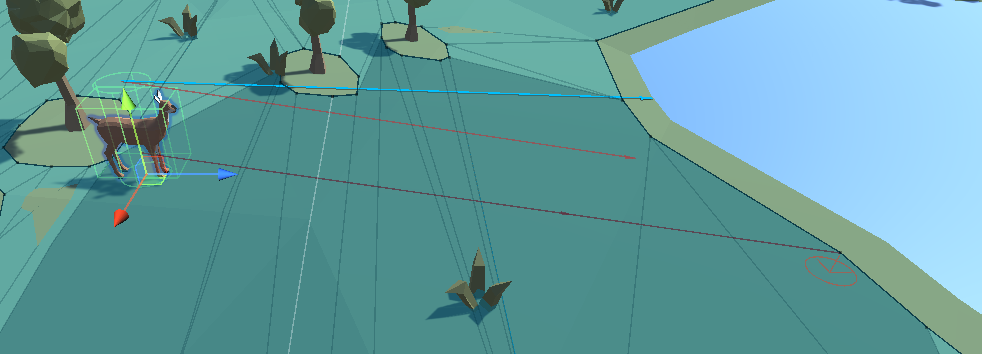
\includegraphics[width=\linewidth]{Deer Drinking.png}
		\caption{A Deer Drinking.}
		\label{fig:Deer Drinking}
	\end{figure}
	
\section{Reproduce}
	In order to test the Reproduce state we spawned two agents of opposite gender and set their reproductive urges to above the threshold. We can see the two agents approach each other and once in range the female spawns a baby. If the agents are significantly far apart they will call again to update the partner (as well as other potential mates) of the current location. By testing in this way we discovered many bugs that may have been missed by just observing the complete simulation, for example, the wolves spawning baby deer, and same gender reproduction. This is shown in \ref{fig:Deer Reproducing}
	
	\begin{figure}
		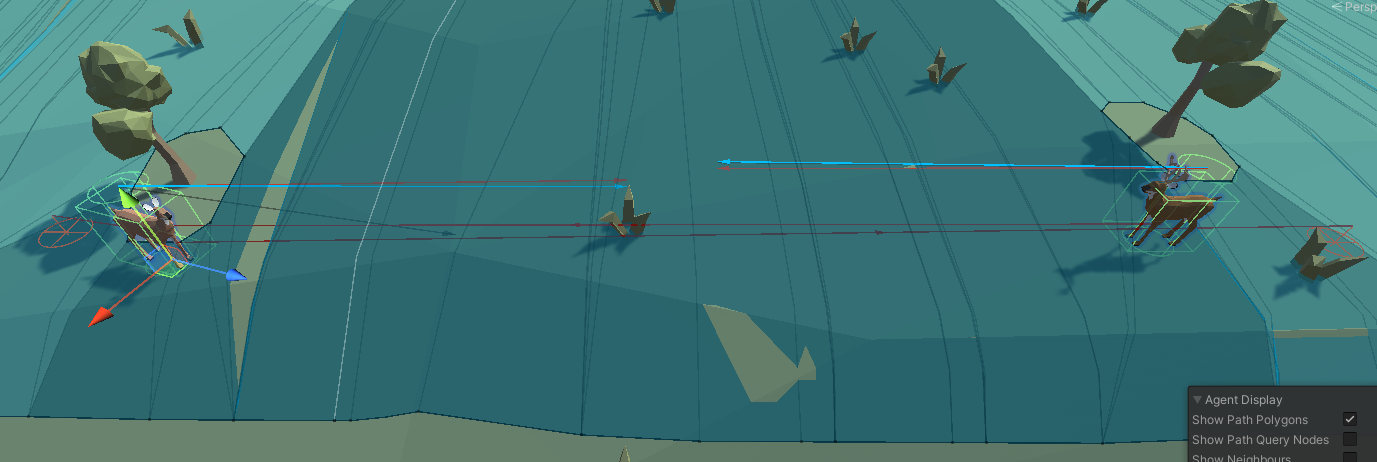
\includegraphics[width=\linewidth]{Deer Reproducing.png}
		\caption{Deer Reproducing.}
		\label{fig:Deer Reproducing}
	\end{figure}
	
\section{Feed}
	In order to test the Feed state we manually set the deer's hunger to below the threshold and place some grass for it to find, making sure it can find what it is supposed to. We also set up situations that we thought may cause issues like targets outside of their navmesh. Using serialized fields we can see that the hunger attribute is successfully updated. This is shown in \ref{fig:Deer Feeding}
	
	\begin{figure}
		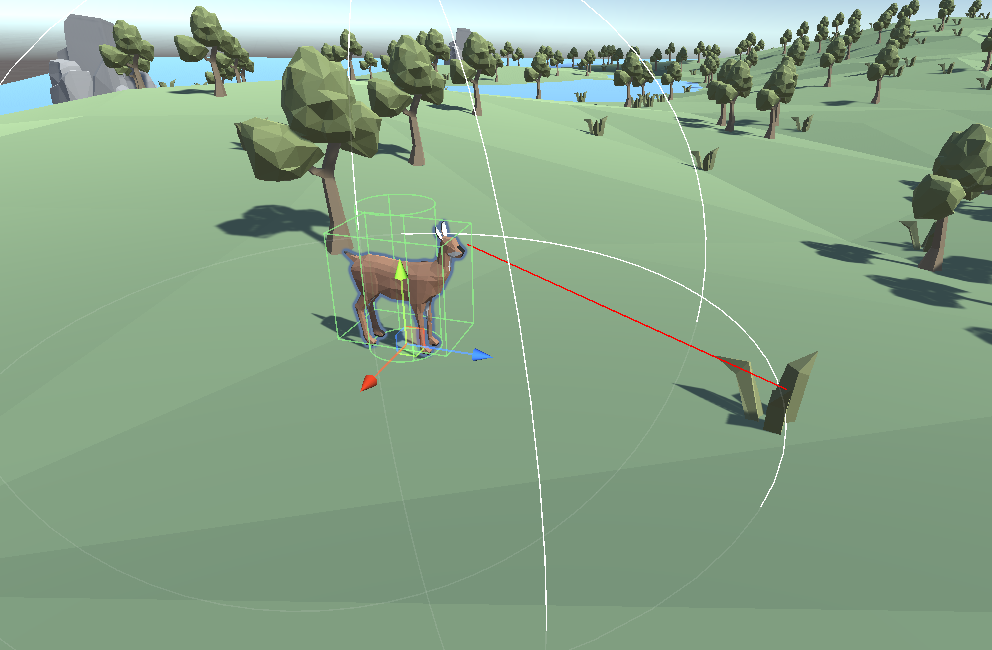
\includegraphics[width=\linewidth]{Deer Feeding.png}
		\caption{A Deer Feeding.}
		\label{fig:Deer Feeding}
	\end{figure}
	
\section{Hunt and Flee}
	In order to test the Hunt and Flee state we placed a deer and a wolf next to each other in the environment and set the wolf's hunger to be below the threshold. This is shown in \ref{fig:Wolf Hunting}
	
	\begin{figure}
		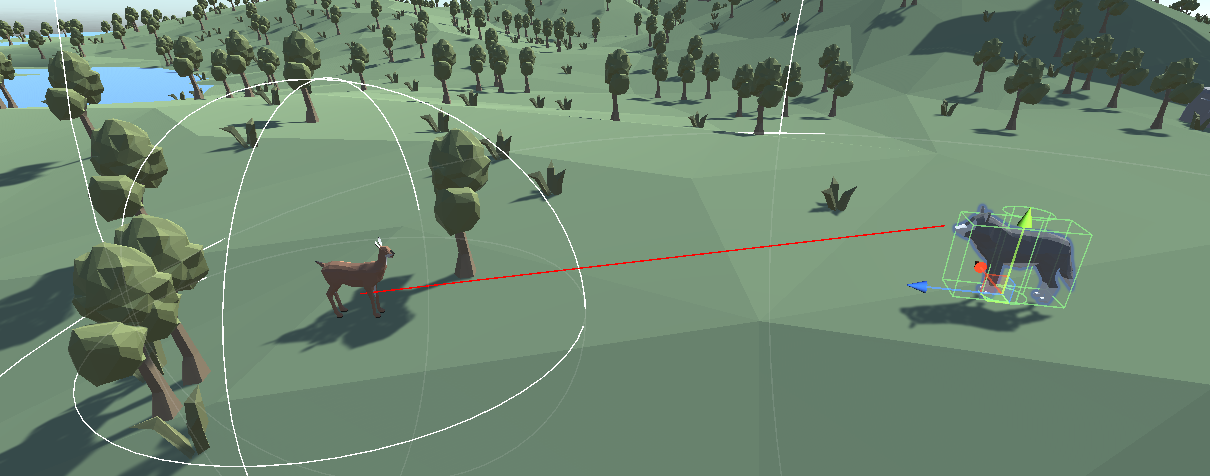
\includegraphics[width=\linewidth]{Wolf Hunting.png}
		\caption{A Wolf Hunting.}
		\label{fig:Wolf Hunting}
	\end{figure}


\chapter{Discussion, conclusion and future work}
	The final product satisfies all of the must category but does not satisfy any of the should category. We had hopes to implement a diploid gene system that would have created differences in agents from the same species across the simulation, and to graph the amounts of different genes as the simulation continued to see which had a better rate of survival. We had also hoped to add a "Smart Decision" system that would have improved how the agents choose which state they should be in and would have increased the amount of activity across the simulation as the "Idle" state caused a lot of stationary agents. This system would have also made the agents better at surviving, leaving less to random chance and giving a better impression of how well the agents could survive the environment based on their behaviour. Another system we wanted to implement was a weighted movement system, this would have replaced any instances of random movement and would have resulted in much more interesting behaviour and opportunities to improve the simulation. This system would have taken into account things like hunting pressure and feeding areas when deciding where the agent should move. In conclusion the ecology simulation produced was not where we had hoped it would be, and essentially ended up being the Minimum Viable Product for this project. 


\bibliographystyle{unsrt}
\bibliography{References}

\chapter*{Contributions}


\end{document}

